\chapter{Mixing, Oscillation, Electric Dipole Moments, and Field Operators}

We begin a little off the advertised subject, with a question about neutrinos. There is evidence that neutrinos have mass and that the neutrino types mix. If the masses are not all the same, how can one type turn into another without violating energy conservation?

The question points to a pattern that occurs throughout quantum mechanics: the states in which a system is prepared or detected need not be the states that diagonalize its Hamiltonian. A state with definite energy only acquires a phase. A prepared state that is a superposition of several energies changes because its components acquire different phases. That distinction will carry us from a double well to neutrino oscillation and spin precession. After an interlude on the electron electric dipole moment, we shall return to second quantization and see the same position--momentum Fourier structure at the operator level.

\section{Mixing as the Real Issue}

Neutrinos need not all have the same mass. The energy eigenstates do not mix with one another; each evolves independently. What we call the \emph{type}, or flavor, of a neutrino is associated with how it is produced and detected, and a flavor state can be a linear combination of mass-energy eigenstates. Schematically,
\begin{equation}
|\text{type}\rangle = \sum_n c_n |E_n\rangle .
\end{equation}
Thus the right statement is not that energy eigenstates change into one another, but that the states called ``electron neutrino'' or ``muon neutrino'' need not themselves be energy eigenstates.

\begin{classroomqa}
\lecturetimestamp{00:00:09}
\audiencequestion{If neutrinos have different masses, how can they mix while energy remains conserved?}
\lecturerresponse{The mass-energy eigenstates do not change into one another. Electron-, muon-, and tau-flavor states are different linear combinations of those eigenstates. Each mass component evolves with its own phase, and interference changes the flavor probabilities without violating energy conservation.}
\end{classroomqa}

There are many examples of this structure. The most visible one begins with a particle in a symmetric double well.

\section{Symmetric Double Well and Approximate Localized States}

Consider a particle moving in a symmetric double-well potential with a high barrier between the two minima. If the barrier were taken to be infinitely high, then the left and right wells would decouple completely. One could solve the left-hand well as though the right-hand well did not exist, and likewise for the right-hand well. The approximate ground-state wavefunctions would then be a left-localized state \(\psi_L\) and a right-localized state \(\psi_R\), both with the same energy \(E\).

In each isolated well the ground state has the familiar qualitative properties: it is smooth, has no nodes, and sits at the lowest possible energy consistent with confinement. Think of the high central barrier as a brick wall. Treating it as infinite is only an approximation, but it gives us a useful pair of localized states from which to begin.

\begin{figure}
\centering
\begin{adjustbox}{max width=\linewidth}
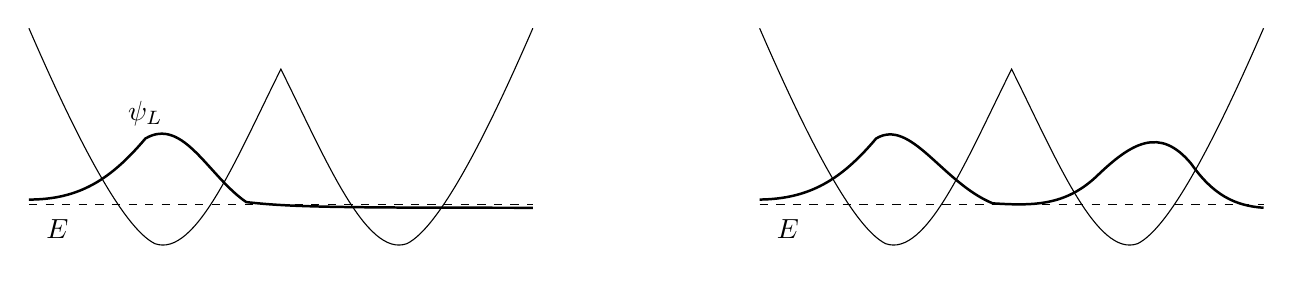
\begin{tikzpicture}[x=0.8cm,y=0.8cm]
\begin{scope}[shift={(-5.8,0)}]
\draw (-4,2.7) .. controls (-3.35,1.2) and (-2.55,-0.45) .. (-2.0,-0.72)
      .. controls (-1.35,-0.95) and (-0.7,0.65) .. (0,2.05)
      .. controls (0.7,0.65) and (1.35,-0.95) .. (2.0,-0.72)
      .. controls (2.55,-0.45) and (3.35,1.2) .. (4,2.7);
\draw[dashed] (-4,-0.10) -- (4,-0.10);
\node at (-3.55,-0.48) {$E$};
\draw[line width=0.9pt] (-4,-0.02) .. controls (-3.2,-0.02) and (-2.7,0.30) .. (-2.15,0.95)
      .. controls (-1.55,1.30) and (-1.15,0.35) .. (-0.55,-0.06)
      .. controls (0.15,-0.14) and (0.9,-0.15) .. (4,-0.15);
\node at (-2.15,1.35) {$\psi_L$};
\end{scope}
\begin{scope}[shift={(5.8,0)}]
\draw (-4,2.7) .. controls (-3.35,1.2) and (-2.55,-0.45) .. (-2.0,-0.72)
      .. controls (-1.35,-0.95) and (-0.7,0.65) .. (0,2.05)
      .. controls (0.7,0.65) and (1.35,-0.95) .. (2.0,-0.72)
      .. controls (2.55,-0.45) and (3.35,1.2) .. (4,2.7);
\draw[dashed] (-4,-0.10) -- (4,-0.10);
\node at (-3.55,-0.48) {$E$};
\draw[line width=0.9pt] (-4,-0.02) .. controls (-3.2,-0.01) and (-2.7,0.30) .. (-2.15,0.95)
      .. controls (-1.6,1.28) and (-1.1,0.25) .. (-0.30,-0.08)
      .. controls (0.35,-0.12) and (0.85,-0.12) .. (1.35,0.35)
      .. controls (1.9,0.88) and (2.35,1.15) .. (2.85,0.55)
      .. controls (3.2,0.05) and (3.55,-0.12) .. (4,-0.15);
\end{scope}
\end{tikzpicture}
\end{adjustbox}
\caption{A clean redraw of the opening board sketches. On the left is the one-sided trial state \(\psi_L\), obtained by pretending the barrier is effectively infinite. On the right the same wavefunction has been continued symmetrically through the barrier, illustrating the small but nonzero leakage that eventually produces the true even ground state.}
\end{figure}

Quantum mechanically, however, the barrier is not truly infinite. The wavefunction in the barrier region is not exactly zero; it is only very small. This tiny leakage is the whole story. It is what converts the left-right approximation into a genuine mixing problem.

\section{Parity Eigenstates and Exponential Level Splitting}

The localized picture is now interrupted by a theorem: if the potential is symmetric, then the exact energy eigenfunctions can be chosen to be either symmetric or antisymmetric under reflection.

\begin{theorem}
If \(V(x)=V(-x)\) in one dimension, then the eigenfunctions of the Hamiltonian may be chosen to satisfy either
\[
\psi(x)=\psi(-x)
\qquad \text{or} \qquad
\psi(x)=-\psi(-x).
\]
\end{theorem}

Now comes the correction. The one-sided states \(\psi_L\) and \(\psi_R\) are neither symmetric nor antisymmetric, so they cannot be exact eigenstates of the full Hamiltonian. They are only good approximate states when the barrier is high. The true eigenstates are the symmetric and antisymmetric combinations,
\begin{align}
\psi_+ &= \frac{\psi_L+\psi_R}{\sqrt{2}},\\
\psi_- &= \frac{\psi_L-\psi_R}{\sqrt{2}}.
\end{align}
Using the notation that will remain on the board, label their energies by
\begin{align}
H\psi_+ &= (E_1-\epsilon)\psi_+,\\
H\psi_- &= (E_1+\epsilon)\psi_-.
\end{align}
The total splitting is therefore
\begin{equation}
\Delta E = (E_1+\epsilon)-(E_1-\epsilon)=2\epsilon .
\end{equation}

\begin{figure}[htbp]
\centering
\includegraphics[width=0.92\linewidth]{lecture_08_frame_02.png}
\caption{The symmetrically continued wavefunction in the double-well potential. Its amplitude is small but nonzero under the barrier, which is the origin of the level splitting.}
\lectureframe{00:06:19}
\end{figure}

\begin{figure}
\centering
\begin{tikzpicture}[x=1cm,y=1cm]
\draw[->] (0,0) -- (0,3);
\node[left] at (0,2.8) {energy};
\draw (-0.35,1.60) -- (0.35,1.60);
\node[left] at (-0.45,1.60) {$\psi_L,\psi_R$};
\node at (1.7,1.60) {$\Longrightarrow$};
\draw (3.0,1.32) -- (3.75,1.32);
\draw (3.0,1.88) -- (3.75,1.88);
\draw[dashed] (2.8,1.60) -- (3.95,1.60);
\node[right] at (3.9,1.32) {$\psi_+,\ E_1-\epsilon$};
\node[right] at (3.9,1.88) {$\psi_-,\ E_1+\epsilon$};
\node[below] at (3.37,1.60) {$E_1$};
\end{tikzpicture}
\caption{The board logic of the tunnel splitting. The approximate left and right states are nearly degenerate, but the exact symmetric and antisymmetric eigenstates are split by a small amount \(2\epsilon\).}
\end{figure}

The ordering of the levels carries the physical point. The symmetric state is slightly lower in energy because it is smoother through the barrier region; allowing the wavefunction to leak and continue symmetrically lowers the energy by a tiny amount. The antisymmetric state is slightly higher because the first excited state in one dimension has one node, and in this symmetric problem that node sits at the midpoint. Extra curvature costs kinetic energy.

The effect is very small, exponentially small in the barrier width and height. We do not need an explicit WKB formula here; the important point is that the splitting is real but tiny. Also remember that the overall sign of a wavefunction carries no physical information. Replacing \(\psi_-\) by \(-\psi_-\) does not change the state.

\section{Time Evolution and Left-Right Oscillation}

Now ask the dynamical question: what happens if we place a particle in the left-hand well? This is the decisive step, because oscillation is the time-dependent face of the same mixing phenomenon.

The inverse relations are
\begin{align}
\psi_L &= \frac{\psi_+ + \psi_-}{\sqrt{2}},\\
\psi_R &= \frac{\psi_+ - \psi_-}{\sqrt{2}}.
\end{align}
So an initially left-localized state is
\begin{equation}
\psi(0)=\psi_L=\frac{\psi_+ + \psi_-}{\sqrt{2}}.
\end{equation}
It is not an energy eigenstate, and therefore it must evolve nontrivially.

We use the standard Schr\"odinger convention \(e^{-iEt}\). A common phase has no observable effect; only the relative phase between the two energy components can move probability from one well to the other.

With that convention,
\begin{equation}
\psi(t)=\frac{1}{\sqrt{2}}\left(e^{-i(E_1-\epsilon)t}\psi_+ + e^{-i(E_1+\epsilon)t}\psi_-\right).
\end{equation}
This is the cleaned version of the board formula. Now factor out the common phase:
\begin{equation}
\psi(t)=\frac{e^{-iE_1 t}}{\sqrt{2}}\left(e^{i\epsilon t}\psi_+ + e^{-i\epsilon t}\psi_-\right).
\end{equation}
One phase now runs one way around the unit circle while the other runs the opposite way. The state changes only because these two phases drift out of step.

To see the left-right oscillation explicitly, substitute the definitions of \(\psi_\pm\):
\begin{align}
\psi(t)
&= \frac{e^{-iE_1 t}}{2}
\left[e^{i\epsilon t}(\psi_L+\psi_R)+e^{-i\epsilon t}(\psi_L-\psi_R)\right] \\
&= \frac{e^{-iE_1 t}}{2}
\left[(e^{i\epsilon t}+e^{-i\epsilon t})\psi_L+(e^{i\epsilon t}-e^{-i\epsilon t})\psi_R\right] \\
&= e^{-iE_1 t}\left[\psi_L\cos(\epsilon t)+i\,\psi_R\sin(\epsilon t)\right].
\end{align}
This is the key worked derivation of the chapter. In the two-state approximation, with \(\psi_L\) and \(\psi_R\) orthonormal, the probabilities are
\begin{equation}
P_L(t)=\cos^2(\epsilon t),
\qquad
P_R(t)=\sin^2(\epsilon t).
\end{equation}
So the system oscillates. At intermediate times it is genuinely in superposition; for example, when \(\epsilon t=\pi/4\), the probabilities on the two sides are equal. The phases evolve continuously, and the localization changes continuously with them.

The blackboard derivation isolates the first time at which the relative sign flips. One asks when
\begin{equation}
e^{-i\epsilon t}=-\,e^{i\epsilon t},
\end{equation}
which is the visible milestone on the board. Multiplying through gives
\begin{equation}
e^{2i\epsilon t}=-1.
\end{equation}
For the first occurrence,
\begin{equation}
2\epsilon t=\pi,
\qquad\text{so}\qquad
t_{L\to R}=\frac{\pi}{2\epsilon}.
\end{equation}

\begin{figure}[htbp]
\centering
\includegraphics[width=0.94\linewidth]{lecture_08_frame_05.png}
\caption{The relative-phase calculation on the board. The two energy components become opposite when \(e^{2i\epsilon t}=-1\), giving the first transfer time \(2\epsilon t=\pi\). The typeset derivation uses one consistent Schr\"odinger-phase convention.}
\lectureframe{00:17:52}
\end{figure}
At that instant,
\begin{equation}
\psi(t_{L\to R}) \propto \frac{\psi_+-\psi_-}{\sqrt{2}}=\psi_R.
\end{equation}
The overall phase is irrelevant. What matters is that the particle initially placed on the left has evolved into the right-localized state. After another equal interval it swings back again. Mixing and oscillation go together.

The equation is unambiguous: small \(\epsilon\) means slow oscillation and a long transfer time. Neither localized state has a definite energy, but the two exact energy components conserve energy and evolve exactly as they should.

\section{Neutrino, Ammonia, and Spin Analogies}

The double well gives us a template for the original neutrino question. A neutrino created together with an electron is called an electron neutrino; one created together with a muon is called a muon neutrino. Those flavor labels describe production and detection channels. The states with definite masses, and hence definite free-particle energies at fixed momentum, form another basis.

In the simplest two-state, maximally mixed caricature,
\begin{equation}
|\nu_e\rangle \sim \frac{|m_1\rangle+|m_2\rangle}{\sqrt{2}},
\qquad
|\nu_\mu\rangle \sim \frac{|m_1\rangle-|m_2\rangle}{\sqrt{2}},
\end{equation}
where the mass eigenstates play the role of \(\psi_+\) and \(\psi_-\), and the flavor states play the role of \(\psi_L\) and \(\psi_R\). Real neutrino mixing uses a nontrivial mixing matrix rather than these equal coefficients, but the mechanism is already visible here.

An electron neutrino is produced in a process involving an electron, just as a particle can be plunked into the left well. For a short flight its two mass components have accumulated almost the same phase, so an interaction still identifies it as electron flavor. Over a long baseline their phases separate. A later charged-current interaction can then produce a muon rather than an electron: the state has acquired a muon-flavor component. Repeating the experiment at different distances or energies reveals the oscillation.

There is no conflict with energy conservation. The mass-energy eigenstates do exactly what eigenstates are supposed to do. It is the flavor superposition that evolves. In the relativistic limit the observable relative phase is governed by mass-squared differences, schematically
\begin{equation}
\Delta\phi_{ij}\simeq \frac{\Delta m_{ij}^{,2}L}{2E}.
\end{equation}
Oscillation therefore shows that not all neutrino masses can be identical; at least two mass eigenstates differ in mass.

\begin{classroomqa}
\lecturetimestamp{00:24:06}
\audiencequestion{What determines the small splitting \(\epsilon\) in the double-well example?}
\lecturerresponse{It depends on the particle mass and on the barrier's height and width. Tunneling is exponentially sensitive to those details, so a modest change in the barrier can produce a large fractional change in \(\epsilon\).}
\end{classroomqa}

\begin{classroomqa}
\lecturetimestamp{00:24:26}
\audiencequestion{Has this oscillation phenomenon actually been observed?}
\lecturerresponse{Yes. Tunneling splittings are observed in ordinary quantum systems, and flavor oscillations are observed for neutrinos. The mechanisms differ microscopically, but both realize the same two-state phase evolution.}
\end{classroomqa}

\begin{classroomqa}
\lecturetimestamp{00:24:34}
\audiencequestion{How is neutrino oscillation connected to neutrino mass?}
\lecturerresponse{The propagating eigenstates have different masses and therefore accumulate different phases. Their interference changes the flavor composition. In a realistic relativistic treatment it is the mass-squared differences, not a literal time-varying mass of one particle, that control the oscillation.}
\end{classroomqa}

\begin{classroomqa}
\lecturetimestamp{00:25:02}
\audiencequestion{Is neutrino mass merely prevailing theory, or is it experimental fact?}
\lecturerresponse{Oscillation is experimental fact, and it requires nonzero mass differences. The absolute mass scale is a separate and more difficult measurement, but the minimal picture in which every neutrino is massless is experimentally excluded.}
\end{classroomqa}

\subsection{Ammonia inversion: a literal barrier}

An ammonia molecule, \(\mathrm{NH}_3\), is trigonal pyramidal: the three hydrogen atoms form a plane and the nitrogen lies on one side of it. There is an equivalent configuration with the nitrogen on the other side. The two localized configurations are not exact stationary states. The nitrogen can tunnel through the hydrogen plane, producing symmetric and antisymmetric energy eigenstates and a small inversion splitting. This is the physical origin of the same mathematics in the ammonia maser.

\begin{classroomqa}
\lecturetimestamp{00:25:11}
\audiencequestion{In ammonia, is the barrier the configuration in which the nitrogen passes through the hydrogen plane?}
\lecturerresponse{Yes. The molecular energy is minimized in either pyramidal configuration, while the planar configuration lies higher. Tunneling through that configuration couples the two sides.}
\end{classroomqa}

\begin{classroomqa}
\lecturetimestamp{00:27:10}
\audiencequestion{What is the corresponding physical barrier between electron and muon neutrinos?}
\lecturerresponse{There is no literal spatial barrier. The analogy is algebraic: an off-diagonal coupling in the neutrino Hamiltonian mixes the flavor basis. In ammonia that coupling arises from tunneling; for neutrinos it is part of the mass and mixing structure.}
\end{classroomqa}

\subsection{Spin precession: mixing without tunneling}

We have already met the same algebra in spin. Take the two states \(|\uparrow_z\rangle\) and \(|\downarrow_z\rangle\). With no magnetic field they are degenerate. Now turn on a magnetic field in the \(x\)-direction. The energy eigenstates are no longer the \(z\)-eigenstates but the \(x\)-polarized states. Using the temporary left--right names from the board,
\begin{align}
|L_x\rangle &= \frac{|\uparrow_z\rangle+|\downarrow_z\rangle}{\sqrt{2}},\\
|R_x\rangle &= \frac{|\uparrow_z\rangle-|\downarrow_z\rangle}{\sqrt{2}}.
\end{align}
These are the direct analogues of \(\psi_+\) and \(\psi_-\). The magnetic moment aligned and antialigned with the field has slightly different energy. If those energies are \(E\mp\epsilon\), then an initially up spin evolves as
\begin{equation}
|\uparrow_z,t\rangle
= e^{-iEt}\left[\cos(\epsilon t)\,|\uparrow_z\rangle
+ i\sin(\epsilon t)\,|\downarrow_z\rangle\right].
\end{equation}
This is the same formula as for the double well, only now the continuous evolution is spin precession about the \(x\)-axis. Starting from \(+z\), the spin passes through transverse directions, reaches \(-z\) after half a precession period, and returns after another half period. A measurement of \(S_z\) still yields only up or down; the continuously changing spin state determines their probabilities. The mechanism does not require tunneling. It requires only that the Hamiltonian be diagonal in a basis different from the preparation basis.

\begin{classroomqa}
\lecturetimestamp{00:32:25}
\audiencequestion{What happens to the tau neutrino in this picture?}
\lecturerresponse{It mixes as well. The real problem has three flavor states and three mass states, so a three-by-three mixing matrix replaces the two-state rotation. The phase-interference principle is unchanged.}
\end{classroomqa}

\begin{classroomqa}
\lecturetimestamp{00:32:57}
\audiencequestion{Immediately after the transverse field is applied, is the spin still up, and can it point toward or away from us?}
\lecturerresponse{At a very short time it is still almost certainly up, with a small down probability. The state precesses continuously around the field axis and passes through the transverse \(\pm y\) directions, while remaining perpendicular to the \(x\)-directed field if it began perpendicular. A measurement along any chosen axis still gives one of that axis's discrete eigenvalues.}
\end{classroomqa}

\begin{classroomqa}
\lecturetimestamp{00:34:30}
\audiencequestion{Is the field chosen weak so that the spin never points along the field?}
\lecturerresponse{No. The geometry follows from precession about the field axis, not from the field's weakness. A weak field merely makes the energy splitting and precession frequency small, giving a slow oscillation analogous to the neutrino example.}
\end{classroomqa}

The strength of neutrino mixing and the small neutrino masses are parameters whose deeper origin is not explained by the minimal Standard Model as originally formulated. Neutrino mass therefore points beyond that minimal model, though the observed scale is very small and may reflect physics at a remote energy scale.

\begin{classroomqa}
\lecturetimestamp{00:36:27}
\audiencequestion{Is oscillation the reason we know neutrinos have mass?}
\lecturerresponse{It is the decisive direct evidence that the propagating components have different masses. If all relevant components were exactly massless and degenerate, they would accumulate no mass-dependent relative phase and there would be no vacuum flavor oscillation of this kind.}
\end{classroomqa}

\begin{classroomqa}
\lecturetimestamp{00:37:57}
\audiencequestion{At half a period, should a neutrino act half like electron flavor and half like muon flavor?}
\lecturerresponse{In the ideal symmetric two-state model, equal probabilities occur at a quarter of the full probability period, while complete conversion occurs at the first maximum. Real three-flavor oscillations have unequal mixing angles, several frequencies, spin-helicity constraints, and matter effects, so complete symmetric conversion is not generic.}
\end{classroomqa}

\begin{classroomqa}
\lecturetimestamp{00:38:36}
\audiencequestion{If the mass components differ, must a solar neutrino's velocity change in order to conserve momentum?}
\lecturerresponse{A flavor state is a coherent superposition of components with fixed masses; its mass is not a classical quantity oscillating in time. In the common equal-momentum description the components have slightly different energies and group velocities, while in an equal-energy description they have slightly different momenta. Both conventions give the same observable oscillation phase when treated consistently.}
\end{classroomqa}

This phase evolution resolved the old solar-neutrino deficit. Early detectors were primarily sensitive to electron neutrinos, so neutrinos that left the Sun as electron flavor could arrive partly as muon or tau flavor and escape that channel. The detailed solar calculation includes three-flavor mixing and matter effects, but the conceptual lesson is already present in the double well: preparation and propagation use different bases.

\section{Interlude: Electric Dipole Moment, Symmetry, and the ``Electron Sphere'' Claim}

Since we are already talking about particle phenomenology, let us take a break from formal mathematics. A popular article described a new electron electric-dipole-moment bound by saying that the electron had been shown to be a sphere. That slogan confuses three different questions: what an electric dipole moment measures, what rotational symmetry means for a quantum state, and what the experiment actually constrained.

\subsection{What was measured?}

What was measured, or rather bounded, is the electric dipole moment of the electron. For separated charges \(\pm q\), the dipole moment is
\begin{equation}
\mathbf d = q\,\boldsymbol{\ell},
\end{equation}
with \(\boldsymbol{\ell}\) the separation vector. A nonzero dipole moment means that the charge distribution is displaced relative to some center.

For the electron, however, the relevant question is not merely whether the charge is off-center in some arbitrary direction. The electron has spin and therefore an axis. It also has a magnetic moment. The physically meaningful question is whether there is a correlation between the displacement of charge and that axis:
\begin{equation}
\mathbf d_e \parallel \boldsymbol{\mu}_e
\qquad \text{or equivalently} \qquad
\mathbf d_e \parallel \mathbf S .
\end{equation}
That correlation is what is meant by the electron's electric dipole moment. Conceptually, one asks whether placing a spin-polarized electron in an electric field splits the two spin orientations:
\begin{equation}
H_{\mathrm{EDM}}=-\mathbf d_e\cdot \mathbf E,
\qquad
\mathbf d_e=d_e\frac{\mathbf S}{|\mathbf S|}.
\end{equation}
The actual tabletop experiment is much subtler than a bare electron sitting between capacitor plates, but this is the symmetry and energy-shift idea it exploits.

\subsection{Why no EDM does not mean sphere}

The first correction is elementary. A body can have no dipole moment and still not be spherical. A centered ellipsoid has as much charge on one side as on the other and therefore no dipole, yet it can have a quadrupole moment. A still more complicated distribution may have neither dipole nor quadrupole while retaining a higher multipole. Measuring one multipole coefficient does not determine an entire shape.

Quantum mechanics makes the word ``shape'' more delicate. Imagine a two-atom, dumbbell-like molecule with an approximately fixed bond length. Ignore radial vibration and keep only rotations. Its rotational states are labeled by angular momentum. If the molecule is bosonic, the lowest rotational state has \(J=0\). Because angular momentum generates rotations,
\begin{equation}
\begin{gathered}
J=0 \quad\Longrightarrow\\
\text{rotationally invariant ground state.}
\end{gathered}
\end{equation}
The quantum state is rotationally invariant even though every
definite-orientation picture looks like a dumbbell. One may describe it as a
coherent superposition of all orientations. Calling the state ``spherical''
is useful for some measurements and misleading for others.

Take a quick snapshot. A snapshot is a measurement of orientation, and a sufficiently sharp orientation measurement leaves the system in a state localized in angle. Such a state cannot also have definite angular momentum. This is the rotational version of the position--momentum uncertainty principle: localizing angle necessarily introduces a spread of angular momenta and therefore rotational excitation.

For a rigid rotor,
\begin{equation}
E_J=\frac{J(J+1)}{2I},
\end{equation}
so the resolving energy is controlled by the moment of inertia \(I\). A gymnasium dumbbell has an enormous \(I\) and fantastically close rotational levels; ordinary light can easily disturb it enough to reveal an orientation. A molecule has wider level spacing. A compact hadron has much wider spacing still. If the probe lacks enough energy to excite the first resolvable rotational structure, repeated measurements see only the rotationally averaged ground state.

A meson can be pictured loosely as a quark--antiquark two-body system. Its first orbital excitations cost hundreds of millions of electron volts or more, far beyond an optical photon. A low-energy probe therefore cannot take a snapshot of the underlying orientation. ``Sphere or not'' is partly a question about which state is prepared and partly a question about the resolution of the apparatus.

The electron sharpens the issue. It is a spin-\(\tfrac12\) particle, not a rotational scalar. A spin-polarized state carries an axis and a magnetic moment. The familiar picture of circulating charge around that axis is only a heuristic---a pointlike Dirac particle is not literally a tiny spinning ball---but it correctly reminds us that the magnetic moment reverses with spin. The EDM question asks whether the electric charge displacement is correlated with that same axis. A null answer does not turn the electron into a classical sphere.

\begin{classroomqa}
\lecturetimestamp{00:57:30}
\audiencequestion{Would displacing part of the electron's charge violate charge quantization?}
\lecturerresponse{No. Charge quantization fixes the total charge. A dipole moment concerns the first spatial moment of that charge distribution, or equivalently an allowed point-particle coupling to the electric field; it does not require a fractional change in total charge.}
\end{classroomqa}

\begin{classroomqa}
\lecturetimestamp{00:58:00}
\audiencequestion{Are electric dipole moments forbidden by quantum field theory?}
\lecturerresponse{Not by quantum field theory itself. They are forbidden when particular discrete symmetries are exact. Once those symmetries are violated, an EDM operator is allowed, although its coefficient may be extremely small.}
\end{classroomqa}

\subsection{Parity and time reversal}

The real content of the EDM discussion is symmetry. Under parity, an electric dipole moment behaves as an ordinary polar vector, while a magnetic moment behaves as an axial vector:
\begin{align}
P:\qquad &\mathbf d_e \to -\mathbf d_e,
&\boldsymbol{\mu}_e \to \boldsymbol{\mu}_e .
\end{align}
Under time reversal, the circulating current that defines the magnetic moment reverses, but a static electric displacement does not:
\begin{align}
T:\qquad &\mathbf d_e \to \mathbf d_e,
&\boldsymbol{\mu}_e \to -\boldsymbol{\mu}_e .
\end{align}
Therefore a nonzero EDM aligned with the electron's spin axis is forbidden by exact parity symmetry and also by exact time-reversal symmetry:
\begin{equation}
(P\ \text{exact}) \Rightarrow \mathbf d_e=0,
\qquad
(T\ \text{exact}) \Rightarrow \mathbf d_e=0.
\end{equation}

The geometry is worth spelling out. A magnetic moment is produced by a loop-like current. Mirror reflection reverses ordinary polar vectors but leaves the axial vector normal to that loop unchanged. A charge displacement along the axis does reverse. Thus an electron with \(\mathbf d_e\) parallel to \(\boldsymbol\mu_e\) would be mirrored into one with the same magnetic orientation but the opposite relation between electric and magnetic moments. If parity were exact and there were only one electron species, the two descriptions would have to represent the same particle; only \(d_e=0\) is consistent.

Time reversal gives the same conclusion in a different way. Running the film backward reverses the current and therefore \(\boldsymbol\mu_e\), but it does not move a static charge displacement. A state with parallel moments becomes one with antiparallel moments. Exact time-reversal symmetry would again require \(d_e=0\).

\begin{figure}[htbp]
\centering
\begin{tikzpicture}[>=Stealth,scale=0.95]
  \node[font=\bfseries] at (1.0,2.25) {original};
  \draw[->,very thick,blue!70!black] (0.65,0) -- (0.65,1.65);
  \draw[->,very thick,red!75!black] (1.35,0) -- (1.35,1.65);
  \node[blue!70!black,below] at (0.65,0) {$\boldsymbol\mu$};
  \node[red!75!black,below] at (1.35,0) {$\mathbf d$};

  \node[font=\bfseries] at (4.5,2.25) {parity};
  \draw[->,very thick,blue!70!black] (4.15,0) -- (4.15,1.65);
  \draw[->,very thick,red!75!black] (4.85,1.65) -- (4.85,0);
  \node[blue!70!black,below] at (4.15,0) {$\boldsymbol\mu$};
  \node[red!75!black,below] at (4.85,0) {$-\mathbf d$};

  \node[font=\bfseries] at (8.0,2.25) {time reversal};
  \draw[->,very thick,blue!70!black] (7.65,1.65) -- (7.65,0);
  \draw[->,very thick,red!75!black] (8.35,0) -- (8.35,1.65);
  \node[blue!70!black,below] at (7.65,0) {$-\boldsymbol\mu$};
  \node[red!75!black,below] at (8.35,0) {$\mathbf d$};
\end{tikzpicture}
\caption{The symmetry test reconstructed from the board argument. Parity reverses the electric dipole but not the axial magnetic moment; time reversal reverses the magnetic moment but not the static electric displacement. Either exact symmetry forbids a permanent EDM parallel to spin.}
\end{figure}

\begin{figure}[htbp]
\centering

\includegraphics[width=0.94\linewidth]{lecture_08_frame_06.png}
\caption{The paired magnetic-axis and charge-displacement sketches during the time-reversal argument. The compact TikZ diagram above isolates the transformation content from the partially erased live board.}
\lectureframe{01:06:10}
\end{figure}

\begin{classroomqa}
\lecturetimestamp{01:06:38}
\audiencequestion{Under time reversal, are both currents and charges reversed?}
\lecturerresponse{Currents reverse because velocities reverse; electric charge itself does not. Charge conjugation \(C\), not time reversal \(T\), reverses the sign of charge.}
\end{classroomqa}

\begin{classroomqa}
\lecturetimestamp{01:07:01}
\audiencequestion{Does the antiunitary character of time reversal mean that nonrelativistic quantum mechanics is not time-reversal invariant?}
\lecturerresponse{No. Antiunitarity is precisely how time reversal is represented consistently in quantum mechanics: it complex-conjugates amplitudes and reverses momenta and spins. Whether a particular Hamiltonian is invariant is a separate question.}
\end{classroomqa}

\begin{classroomqa}
\lecturetimestamp{01:07:19}
\audiencequestion{Does an EDM discussion require the electron to have a finite volume rather than be pointlike?}
\lecturerresponse{No. A point-particle effective Hamiltonian can contain \(-d_e\,\widehat{\mathbf S}\!\cdot\!\mathbf E\). Experiment asks whether opposite spin orientations acquire different electric-field energies; it need not resolve a literal extended charge cloud.}
\end{classroomqa}

Parity is not a symmetry of the weak interactions; it is violated as strongly as possible in their chiral couplings. Time reversal is also not exact, but the known violation in the Standard Model feeds into the electron EDM only at an extraordinarily small level. One can calculate a nonzero Standard-Model contribution, yet it lies far below the sensitivity discussed here. A null result is therefore consistent with the Standard Model while cutting into extensions---supersymmetry and other new interactions, for example---that can generate much larger time-reversal violation.

The basic experimental thought is simple. A magnetic field reveals a magnetic dipole by splitting spin orientations. An electric field would reveal an EDM by an additional spin-correlated energy shift. Real precision experiments use atoms or molecules, long coherent precession times, reversals of applied fields, and careful control of systematics rather than an isolated electron in a naive apparatus.

\begin{classroomqa}
\lecturetimestamp{01:11:02}
\audiencequestion{Was the EDM search a high-energy collision experiment or an experiment with material objects?}
\lecturerresponse{It was precision tabletop physics using electrons bound in a controlled atomic or molecular environment together with electric and magnetic fields. Its energy is low, but its sensitivity to tiny symmetry-violating shifts probes high-energy new physics indirectly.}
\end{classroomqa}

\begin{classroomqa}
\lecturetimestamp{01:12:21}
\audiencequestion{Does the null result constrain which modifications of the Standard Model remain viable?}
\lecturerresponse{Yes in principle: every model predicts a coefficient and therefore occupies some parameter region. The detailed numerical exclusion requires a specialist calculation, but the general logic is firm---agreement with the Standard Model at higher precision leaves less room for alternatives that predict a large EDM.}
\end{classroomqa}

\begin{classroomqa}
\lecturetimestamp{01:13:09}
\audiencequestion{Is time-reversal symmetry required for conservation of quantum information?}
\lecturerresponse{No. Unitary time evolution conserves information even when a Hamiltonian is not invariant under \(T\). A particle in a fixed magnetic field is a familiar example: the field selects an orientation in time-reversed movies unless the field is reversed too, yet the quantum evolution remains unitary. Under the usual assumptions of local Lorentz-invariant quantum field theory, the combined \(CPT\) transformation is a symmetry, but that is not what guarantees unitarity.}
\end{classroomqa}

The break can now end. The null measurement says that the electron has no detected EDM at the stated sensitivity. It does not say that the electron is a sphere, and it does not overthrow the Standard Model; it makes some proposed departures from that model harder to sustain.

\section{Return to Second Quantization: Fourier Transforms, Momentum Modes, and Locality}

We were doing second quantization. Let us restart gently, with a familiar fact about ordinary single-particle wavefunctions, and then lift it to operators. The connection with Fourier transforms is exact and simple.

\subsection{From Position Space to Momentum Space}

Lower-case \(\psi\), not capital \(\Psi\), is the wavefunction of a single particle. In position space,
\begin{equation}
P(x)=|\psi(x)|^2
\end{equation}
is the probability density to find the particle at position \(x\). The momentum-space wavefunction is its Fourier transform,
\begin{equation}
\tilde{\psi}(p)=\int dx\,\psi(x)\,\frac{e^{-ipx}}{\sqrt{2\pi}},
\end{equation}
and the inverse relation is
\begin{equation}
\psi(x)=\int dp\,\tilde{\psi}(p)\,\frac{e^{ipx}}{\sqrt{2\pi}}.
\end{equation}
Then
\begin{equation}
P(p)=|\tilde{\psi}(p)|^2
\end{equation}
is the probability density for momentum \(p\).

We use \(\hbar=1\). The two transforms are inverses: knowing either wavefunction determines the other, while their absolute squares answer different measurement questions.

For a free particle,
\begin{equation}
H=\frac{p^2}{2m},
\end{equation}
so momentum eigenstates are also energy eigenstates, and their position-space wavefunctions are plane waves,
\begin{equation}
\psi_p(x)\propto e^{ipx}.
\end{equation}
This is the point of departure for the second-quantized version.

\begin{figure}[htbp]
\centering

\includegraphics[width=0.94\linewidth]{lecture_08_frame_07.png}
\caption{The position--momentum Fourier pair for a one-particle wavefunction. The distinction between lower-case \(\psi\) and the capital field operator introduced next is essential.}
\lectureframe{01:20:00}
\end{figure}

\subsection{Field operators in position and momentum space}

Now return to the field operator. On the blackboard its annihilation and creation pieces are written as \(\Psi_-(x)\) and \(\Psi_+(x)\). Keeping that notation for a moment,
\begin{align}
\Psi_-(x) &= \sum_i a_i\,\psi_i(x),\\
\Psi_+(x) &= \sum_i a_i^\dagger\,\psi_i^*(x).
\end{align}
Here \(\psi_i(x)\) is the ordinary one-particle wavefunction of the \(i\)-th mode, while \(a_i\) and \(a_i^\dagger\) annihilate and create particles in that mode. From this point on it is convenient to rename
\[
\Psi(x)\equiv \Psi_-(x),
\qquad
\Psi^\dagger(x)\equiv \Psi_+(x).
\]

For a free particle the discrete mode label \(i\) is replaced by the continuous momentum label \(p\). Using the plane waves \(e^{ipx}\), one obtains the standard reconstructed formulas
\begin{align}
\Psi(x) &= \int \frac{dp}{\sqrt{2\pi}}\,a(p)\,e^{ipx},\\
\Psi^\dagger(x) &= \int \frac{dp}{\sqrt{2\pi}}\,a^\dagger(p)\,e^{-ipx}.
\end{align}
These are the field-operator analogues of the ordinary Fourier transform. They can be inverted exactly as before:
\begin{align}
a(p) &= \int \frac{dx}{\sqrt{2\pi}}\,\Psi(x)\,e^{-ipx},\\
a^\dagger(p) &= \int \frac{dx}{\sqrt{2\pi}}\,\Psi^\dagger(x)\,e^{ipx}.
\end{align}
The factors of \(1/\sqrt{2\pi}\) are a convention chosen so that the forward and inverse transforms have the same normalization.

The conceptual content is straightforward. \(\Psi^\dagger(x)\) creates a particle at position \(x\), while \(a^\dagger(p)\) creates a particle with momentum \(p\). Position-space and momentum-space creation operators are Fourier conjugates of one another, just as \(\psi(x)\) and \(\tilde{\psi}(p)\) are Fourier conjugates in ordinary quantum mechanics.

If no particle of momentum \(p\) is present, \(a(p)\) annihilates the state. If particles of that momentum are present, it removes one with the usual occupation-number coefficient. Likewise, \(\Psi(x)\) removes a particle at \(x\), understood distributionally or after smearing into a wavepacket. Each particle species requires its own field operator; one field cannot create every kind of particle.

\subsection{Bosonic commutators and the independence of separated measurements}

The next fact can be derived directly from the definitions. For bosons,
\begin{equation}
[a_i,a_j^\dagger]=\delta_{ij},
\qquad
[a_i,a_j]=0,
\qquad
[a_i^\dagger,a_j^\dagger]=0.
\end{equation}
The continuum version is
\begin{equation}
[a(p),a^\dagger(p')]=\delta(p-p').
\end{equation}
Now compute the equal-time field commutator from the discrete expansion:
\begin{align}
[\Psi(x),\Psi^\dagger(y)]
&= \sum_{i,j}\psi_i(x)\psi_j^*(y)\,[a_i,a_j^\dagger] \\
&= \sum_i \psi_i(x)\psi_i^*(y) \\
&= \delta(x-y),
\end{align}
where the last step uses completeness of the one-particle basis. Likewise,
\begin{equation}
[\Psi(x),\Psi(y)]=0,
\qquad
[\Psi^\dagger(x),\Psi^\dagger(y)]=0.
\end{equation}

\begin{figure}[htbp]
\centering

\includegraphics[width=0.94\linewidth]{lecture_08_frame_08.png}
\caption{The mode commutator and its position-space counterpart on the board. Completeness turns \(\delta_{ij}\) into the spatial delta distribution \(\delta(x-y)\).}
\lectureframe{01:31:00}
\end{figure}

The important point is not merely that \(\Psi\) is non-Hermitian. Define Hermitian quadratures
\begin{equation}
Q(x)=\frac{\Psi(x)+\Psi^\dagger(x)}{\sqrt{2}},
\qquad
P(x)=\frac{\Psi(x)-\Psi^\dagger(x)}{i\sqrt{2}}.
\end{equation}
Their same-point commutator inherits the delta distribution. Thus the two local quadratures are conjugate in the same sense that position and momentum are conjugate. Trying to sharpen one produces uncertainty in the other.

\begin{classroomqa}
\lecturetimestamp{01:32:03}
\audiencequestion{What does the delta function mean when \(x=y\)? Is the commutator large everywhere?}
\lecturerresponse{The delta is a distribution, not an ordinary function with a finite point value. It vanishes for separated arguments and gives a finite result only after integration against a test function. Smearing the fields over a finite detector region turns the formal same-point singularity into the usual finite canonical commutator of two modes.}
\end{classroomqa}

For \(x\neq y\), however, the equal-time commutator vanishes. Operations localized in two disjoint regions can be performed independently: measuring the field here does not give the field there a quantum kick. This is the nonrelativistic equal-time precursor of relativistic microcausality. In a relativistic theory, physical local observables commute at spacelike separation, where no light signal can connect the two events.

The contrast with noncommuting observables is familiar. Since \([x,p]=i\), a precise position measurement disturbs momentum, and a precise momentum state spreads in position. Since different spin components fail to commute, preparing one component sharply makes another uncertain. A nonzero commutator between separated local observables would analogously mean that an operation in one region disturbs the other, contradicting the required causal independence.

\begin{classroomqa}
\lecturetimestamp{01:37:51}
\audiencequestion{Do EPR and entanglement experiments show that a measurement here has an effect on a distant measurement?}
\lecturerresponse{They show correlations, not a controllable causal influence. Entangled outcomes violate classical factorization, but the local statistics at the distant detector cannot be changed by choosing or performing a measurement here. Commutation of spacelike-separated observables is the operator statement behind that no-signalling independence.}
\end{classroomqa}

Next time the algebra changes. Fermion creation and annihilation operators satisfy anticommutation relations. Taken naively, fermion fields at separated points do not commute, so the fields themselves cannot be interpreted as directly measurable bosonic observables. Physical fermionic observables are even combinations---densities, currents, stress tensors---and those local observables recover the required spacelike commutativity. That is the entry point to the fermion version of second quantization.
